\FloatBarrier
\begin{figure}[htb]
\centering
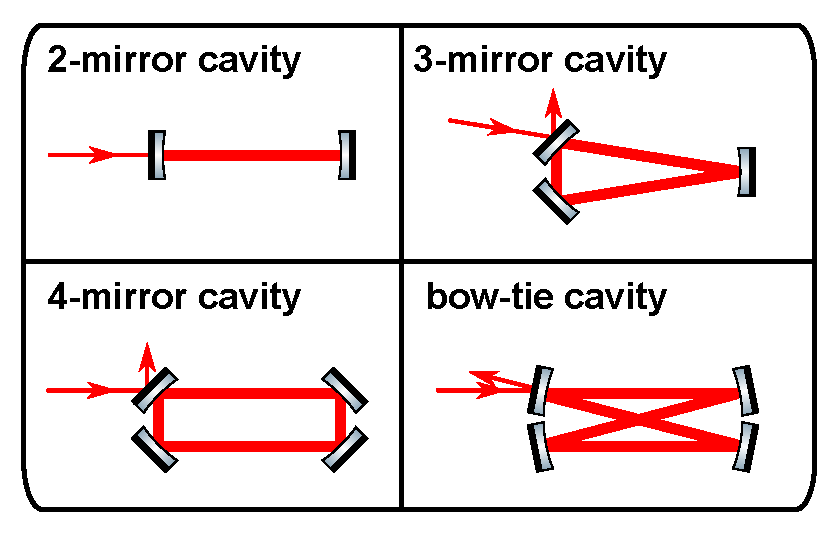
\includegraphics[width=0.5\textwidth]{./Sec_Optics/cavity-designs.pdf}
\caption{Four geometries were analysed from the scattering point of view.}
\label{fig:sc_geometry}
\end{figure}
\paragraph{Choosing the optical layout of the filter cavity}\label{subsec:fcscattering}

%\emph{Author(s): K. Kokeyama, A. Freise, H. L{\"u}ck}

The Einstein Telescope required two 10\,km long and one comparatively
short (several hundred meters long) filter cavities per detector. 
Such filter cavities provide the correct frequency dependence for the injected squeezing state
in order to obtain broad band quantum noise suppression in the main interferometer.
The light reflected off these cavities needs to be injected into the
interferometer dark ports. In principle any cavity geometry can 
provide the correct filtering, however, practical concerns will 
put constraints on the geometry. %In this section we briefly discuss
%these issues, while a selection of the cavity geometry has not been done at this stage.
The four cavity geometries depicted in Fig.~\ref{fig:sc_geometry} are
possible candidates;
the following advantages and disadvantages follow directly from the
geometry (given a long baseline):
\begin{itemize} 
\item the 2-mirror cavity has the advantage of using only two mirrors but
  in order to extract the reflected beam, polarising optics are
  required which introduce additional optical losses and phase noise
\item the 3-mirror cavity provides the reflected beam without the need
  for extra optics. However, the small angle between the beams at the
  far right mirror means that the setup is more sensitive to small
  angle scattering, a problem which has been seen for example in the
  triangular input mode cleaner cavity of VIRGO. Another problem is
  that the large angle of incidence on the two left mirrors requires
  the mirrors to be significant larger compared to the 2-mirror setup.
  of the 10\,km long linear arm cavities. Since the ET optical design is 
  assuming the largest available mirrors being used for the linear arm cavity, this filter
  cavity geometry can be excluded. 
\item the rectangular 4-mirror setup also has the problem of requiring
  larger mirrors due to the angle of incidence.
\item The bow-tie cavity can separate the reflected beam from the
  injected one and does not feature large angles of
  incidence so that the mirror sizes are similar to those of a linear cavity. However, it 
  is sensitive to small angle scattering.
\end{itemize}

% motivation

A detailed study of scattering in the main interferometer and the
filter cavities has not been done yet. 
In Appendix~\ref{app:scatter} we provide a first analysis of the
amount of scattering between the suspended optics itself and conclude
that this effect can be ignored in the selection of the cavity geometry. 






% memo
% mirror surface and scattering
% BRDF
% 4 topologies were compared
% you have to be careful for the rectangular cavity due to the diagonal path
% possible scattering path such as direct back scattering, the effect
% baffles
% two mirror cavity's back scattering? 